% This work is licensed under the GNU aGPL v3 by apehex
% https://github.com/apehex/

\documentclass[11pt,fleqn,oneside]{book} % Default font size and left-justified equations

\usepackage{listofitems} % for \readlist to create arrays
% =======================================================================================
% Global settings
\newcommand{\AUTHOR}{Federico Brancasi}
\newcommand{\CLIENT}{Client Name}
\newcommand{\DATE}{\today}
\newcommand{\VERSION}{0.2.1}
\newcommand{\TITLE}{Deep Learning}
\newcommand{\SUBTITLE}{University of Trento}
\newcommand{\SUBJECT}{Demo}
\newcommand{\URL}{https://github.com/federicobrancasi}

\renewcommand{\SUBJECT}{\href{https://forta.org}{\color{white}Forta.org}}
%%%%%%%%%%%%%%%%%%%%%%%%%%%%%%%%%%%%%%%%%
% By Apehex
% github.com/apehex
%
% Built upon the The Legrand Orange Book by:
% Mathias Legrand (legrand.mathias@gmail.com)
%
% License:
% CC BY-NC-SA 3.0 (http://creativecommons.org/licenses/by-nc-sa/3.0/)
%
%%%%%%%%%%%%%%%%%%%%%%%%%%%%%%%%%%%%%%%%%

%------------------------------------------------------------------------------
%   GENERIC
%------------------------------------------------------------------------------

% ALL GENERIC FEATURES --------------------------------------------------------
%%%%%%%%%%%%%%%%%%%%%%%%%%%%%%%%%%%%%%%%%
% By Apehex
% github.com/apehex
%
% Built upon the The Legrand Orange Book by:
% Mathias Legrand (legrand.mathias@gmail.com)
%
% License:
% CC BY-NC-SA 3.0 (http://creativecommons.org/licenses/by-nc-sa/3.0/)
%
%%%%%%%%%%%%%%%%%%%%%%%%%%%%%%%%%%%%%%%%%

%------------------------------------------------------------------------------
%   GENERIC
%------------------------------------------------------------------------------

% THEMES ----------------------------------------------------------------------
%----------------------------------------------------------------------------------------
%   SOLVE CONFLICTS
%----------------------------------------------------------------------------------------
\PassOptionsToPackage{table}{xcolor}

%----------------------------------------------------------------------------------------
%   COLORS
%----------------------------------------------------------------------------------------
\usepackage[table, usenames,dvipsnames]{xcolor} % Required for specifying colors by name
\usepackage{pagecolor} % dark theme

\colorlet{myred}{red!80!black}
\colorlet{myblue}{blue!80!black}
\colorlet{mybluee}{myblue!80!black}
\colorlet{mygreen}{green!60!black}
\colorlet{myorange}{orange!70!red!60!black}
\colorlet{mydarkred}{red!30!black}
\colorlet{mydarkblue}{blue!40!black}
\colorlet{mydarkgreen}{green!30!black}

%----------------------------------------------------------------------------------------
%   MAKE BOLD STAND OUT
%----------------------------------------------------------------------------------------
\let\oldtextbf\textbf

%----------------------------------------------------------------------------------------
%   DARK THEME
%----------------------------------------------------------------------------------------
\newcommand{\togglethemedark}{
%----------------------------------------------------------------------------------------
\colorlet{accent}{orange}
\colorlet{fg}{white}
\colorlet{fgalt}{lightgray}
\colorlet{fgacc}{white}
\colorlet{bg}{black}
\colorlet{bgalt}{darkgray}
\colorlet{bgacc}{orange}
\colorlet{border}{white}
\colorlet{borderalt}{lightgray}
\colorlet{borderacc}{orange}
%----------------------------------------------------------------------------------------
\pagecolor{bg}
\color{fgalt}
\renewcommand{\textbf}[1]{\oldtextbf{\color{fg}##1}}
}

%----------------------------------------------------------------------------------------
%   LIGHT THEME
%----------------------------------------------------------------------------------------
\newcommand{\togglethemelight}{
%----------------------------------------------------------------------------------------
\colorlet{accent}{orange}
\colorlet{fg}{black}
\colorlet{fgalt}{darkgray}
\colorlet{fgacc}{black}
\colorlet{bg}{white}
\colorlet{bgalt}{lightgray}
\colorlet{bgacc}{orange}
\colorlet{border}{black}
\colorlet{borderalt}{darkgray}
\colorlet{borderacc}{orange}
%----------------------------------------------------------------------------------------
\pagecolor{bg}
\color{fgalt}
\renewcommand{\textbf}[1]{\oldtextbf{\color{fg}##1}}
}

%----------------------------------------------------------------------------------------
%   FORTA THEME
%----------------------------------------------------------------------------------------
\newcommand{\togglethemeforta}{
%----------------------------------------------------------------------------------------
\colorlet{accent}{white}
\colorlet{fg}{white}
\colorlet{fgalt}{lightgray}
\colorlet{fgacc}{black}
\colorlet{bg}{black}
\colorlet{bgalt}{darkgray}
\colorlet{bgacc}{white}
\colorlet{border}{white}
\colorlet{borderalt}{lightgray}
\colorlet{borderacc}{white}
%----------------------------------------------------------------------------------------
\pagecolor{bg}
\color{fgalt}
\renewcommand{\textbf}[1]{\oldtextbf{\color{fg}##1}}
}


%----------------------------------------------------------------------------------------
%   DL THEME
%----------------------------------------------------------------------------------------
\newcommand{\togglethemedl}{
%----------------------------------------------------------------------------------------
\colorlet{accent}{black}
\colorlet{fg}{black}
\colorlet{fgalt}{darkgray}
\colorlet{fgacc}{white}
\colorlet{bg}{white}
\colorlet{bgalt}{lightgray}
\colorlet{bgacc}{black}
\colorlet{border}{black}
\colorlet{borderalt}{darkgray}
\colorlet{borderacc}{black}
%----------------------------------------------------------------------------------------
\pagecolor{bg}
\color{fgalt}
\renewcommand{\textbf}[1]{\oldtextbf{\color{fg}##1}}
}

\togglethemedl

% GEOMETRY --------------------------------------------------------------------
\usepackage{calc} % coordinate calculations

% PAGE LAYOUT -----------------------------------------------------------------
%----------------------------------------------------------------------------------------
%   PARAGRAPH FORMATING
%----------------------------------------------------------------------------------------

\setlength{\parindent}{0pt}
\setlength{\parskip}{12pt}

%----------------------------------------------------------------------------------------
%   FLOAT LAYOUT
%----------------------------------------------------------------------------------------

\renewcommand{\topfraction}{0.9}    % max fraction of floats at top
\renewcommand{\bottomfraction}{0.8} % max fraction of floats at bottom

%   Parameters for TEXT pages (not float pages):
\setcounter{topnumber}{2}
\setcounter{bottomnumber}{2}
\setcounter{totalnumber}{8}     % 2 may work better
\setcounter{dbltopnumber}{2}    % for 2-column pages
\renewcommand{\dbltopfraction}{0.9} % fit big float above 2-col. text
\renewcommand{\textfraction}{0.07}  % allow minimal text w. figs

%   Parameters for FLOAT pages (not text pages):
\renewcommand{\floatpagefraction}{0.7}  % require fuller float pages
\renewcommand{\dblfloatpagefraction}{0.7}   % require fuller float pages

% FONTS -----------------------------------------------------------------------
\usepackage{fontspec} % import new fonts
\usepackage[english]{babel}

%----------------------------------------------------------------------------------------
%   SPACING
%----------------------------------------------------------------------------------------

\usepackage{microtype}

%----------------------------------------------------------------------------------------
%   ADD BOLD + ITALIC
%----------------------------------------------------------------------------------------

\newfontfamily\inconsolatafontfamily[
    Path=template/generic/fonts/inconsolata/,
    Ligatures=TeX,
    Scale=MatchUppercase,
    UprightFont = *.otf,
    BoldFont = *-Bold.otf,
    ItalicFont = *-Italic.otf,
    BoldItalicFont = *-BoldItalic.otf
]{Inconsolata-LGC}

%----------------------------------------------------------------------------------------
%   FAMILY DEFAULTS
%----------------------------------------------------------------------------------------

% \setmonofont{\inconsolatafontfamily}
% \renewcommand*{\familydefault}{\ttdefault}

%----------------------------------------------------------------------------------------
%   HEADINGS
%----------------------------------------------------------------------------------------

\let\headingfontfamily\inconsolatafontfamily

% TITLES ----------------------------------------------------------------------
\usepackage{titlesec}

%----------------------------------------------------------------------------------------
%   SECTION NUMBERING IN THE MARGIN
%----------------------------------------------------------------------------------------

\newcommand{\autodot}{.} % separate title numbers with dots
\newcommand*{\numberinmargin}[3]{\makebox[0pt][r]{\textcolor{#3}{\fontsize{#2}{#2}\selectfont\headingfontfamily\bfseries\selectfont#1\autodot}\hskip\marginparsep}}

%----------------------------------------------------------------------------------------
%   LAYOUT
%----------------------------------------------------------------------------------------

\titlespacing*{\chapter}{0pt}{-30pt}{20pt}

\titlespacing*{\paragraph}{0pt}{3.25ex plus 1ex minus .2ex}{1.5ex plus .2ex}

%----------------------------------------------------------------------------------------
%   FORMAT
%----------------------------------------------------------------------------------------

\titleformat{\chapter}[hang]
  {\normalfont\huge\headingfontfamily\bfseries\selectfont\color{accent}}
  {\numberinmargin{\thechapter}{24}{accent}}
  {0pt}
  {\MakeUppercase}

\titleformat{\section}
  {\normalfont\large\headingfontfamily\bfseries\selectfont\color{fg}}
  {\numberinmargin{\thesection}{16}{accent}}
  {0pt}
  {\MakeUppercase}

\titleformat{\subsection}
  {\normalfont\normalsize\headingfontfamily\bfseries\selectfont\color{fg}}
  {\numberinmargin{\thesubsection}{12}{fg}}
  {0pt}
  {}

\titleformat{\subsubsection}
  {\normalfont\small\headingfontfamily\bfseries\selectfont\color{fg}}
  {\numberinmargin{\thesubsubsection}{10}{fg}}
  {0pt}
  {}

%----------------------------------------------------------------------------------------
%   SPECIAL TITLE
%----------------------------------------------------------------------------------------

\renewcommand{\paragraph}[1]{%
  \par\vspace{3.25ex plus 1ex minus .2ex}%
  \noindent\hspace*{-4cm}\colorbox{bgacc}{%
    \hspace*{4cm}\normalfont\huge\headingfontfamily\selectfont\color{fgacc}\uppercase{#1}
  }%
  \par\nobreak\vspace{1.5ex plus .2ex}%
}

% MATH ------------------------------------------------------------------------
\usepackage{amsmath,amsfonts,amssymb,amsthm} % For math equations, theorems, symbols, etc

\usepackage{tikz}
\usetikzlibrary{calc}
\newcommand{\tikzmarkk}[1]{\tikz[baseline,remember picture] \coordinate (#1) {};}

\usepackage{algorithm}
\usepackage{algorithmic}

% \usepackage{nccmath}
% LINKS -----------------------------------------------------------------------
\usepackage{hyperref}
\usepackage{bookmark}
\usepackage[all]{hypcap} % moves the ref jumping points to the top of images (instead of the caption)

%----------------------------------------------------------------------------------------
%   HYPERLINKS IN THE DOCUMENTS
%----------------------------------------------------------------------------------------
\hypersetup{
hidelinks,
% backref=true,
% pagebackref=true,
% hyperindex=true,
colorlinks=true,
breaklinks=true,
urlcolor=accent,
% bookmarks=true,
bookmarksopen=false,
pdftitle={\TITLE},
pdfauthor={\AUTHOR},
pdfsubject={\texorpdfstring{\SUBJECT}{}},
}

\bookmarksetup{
open,
numbered,
addtohook={%
\ifnum\bookmarkget{level}=0 % chapter
\bookmarksetup{bold}%
\fi
\ifnum\bookmarkget{level}=-1 % part
\bookmarksetup{color=accent,bold}%
\fi
}
}

%----------------------------------------------------------------------------------------
%   BOLD HREF
%----------------------------------------------------------------------------------------

\let\oldhref\href
\renewcommand{\href}[2]{\oldhref{#1}{\headingfontfamily\textbf{#2}}}

% LISTS -----------------------------------------------------------------------
\usepackage{enumitem} % Customize lists

%----------------------------------------------------------------------------------------
%   BULLET POINTS
%----------------------------------------------------------------------------------------

\setlist{nolistsep} % Reduce spacing between bullet points and numbered lists
\setlist[itemize]{leftmargin=4mm}
\setlist[enumerate]{leftmargin=4mm}

%----------------------------------------------------------------------------------------
%   DESCRIPTIONS
%----------------------------------------------------------------------------------------

% \newlength{\desclabelwidth}
% \setlength{\desclabelwidth}{4cm} % default value

% \renewenvironment{description}[1][4cm]
% {\setlength{\desclabelwidth}{#1}
% \begin{list}{}{
%     \renewcommand*{\makelabel}[1]{\bfseries##1\hspace{\desclabelwidth}}
%     \setlength{\itemsep}{0pt}
%     \setlength{\parsep}{0pt}
%     \setlength{\labelsep}{0pt}
%     \setlength{\leftmargin}{0pt}
%     \setlength{\itemindent}{\desclabelwidth}}}
% {\end{list}}

% CODE ------------------------------------------------------------------------
\usepackage{listings}

\input{template/generic/syntax/solidity}

% HEADERS ---------------------------------------------------------------------
\usepackage{fancyhdr} % Required for header and footer configuration

%----------------------------------------------------------------------------------------
%   PAGE HEADERS
%----------------------------------------------------------------------------------------

\fancypagestyle{plain}{%
    % Clear all headers and footers
    \fancyhf{}

    % Remove horizontal line in the header
    \renewcommand{\headrulewidth}{0pt}

    % Page number centered at the bottom
    \fancyfoot[C]{\thepage}
}

\fancypagestyle{fancy}{%
    % Clear all headers and footers
    \fancyhf{}

    % Remove horizontal line in the header
    \renewcommand{\headrulewidth}{0pt}

    % Page number centered at the bottom
    \fancyfoot[C]{\thepage}
}

% BOXES -----------------------------------------------------------------------
\usepackage[most]{tcolorbox}

%----------------------------------------------------------------------------------------
%   HIGHLIGHT ENVIRONMENT
%----------------------------------------------------------------------------------------

\newtcolorbox{highlight}{
  colback=bg,
  colframe=accent,
  coltext=fg,
  boxrule=2pt,
  boxsep=4pt,
  arc=0pt,
  outer arc=0pt
}

%----------------------------------------------------------------------------------------
%   REMARK ENVIRONMENT
%----------------------------------------------------------------------------------------

\newtcolorbox{remark}{
  colback=bg,
  colframe=accent,
  coltext=fg,
  boxrule=0pt,
  leftrule=2pt,
  boxsep=4pt,
  arc=0pt,
  outer arc=0pt,
}

%----------------------------------------------------------------------------------------
%   OUTLINE ENVIRONMENT
%----------------------------------------------------------------------------------------

\newtcolorbox{outline}[1][4pt]{
  enhanced,
  colback=bg,
  colframe=bg, % To essentially hide the frame, but we will draw the corners manually
  coltext=fg,
  boxrule=0pt,
  boxsep=#1,
  arc=0pt,
  outer arc=0pt,
  overlay={
    % Top left corner
    \draw[accent,line width=2pt] 
      (frame.north west) -- ++(0,-0.25*\tcbtextheight)
      (frame.north west) -- ++(0.25*\tcbtextwidth,0);
    % Bottom right corner
    \draw[accent,line width=2pt]
      (frame.south east) -- ++(0,0.25*\tcbtextheight)
      (frame.south east) -- ++(-0.25*\tcbtextwidth,0);
  }
}

% CAPTIONS --------------------------------------------------------------------
\usepackage{caption}

%----------------------------------------------------------------------------------------
%   COMMON
%----------------------------------------------------------------------------------------

\DeclareCaptionFont{fg}{\color{fg}}
\DeclareCaptionFont{accent}{\color{accent}}

%----------------------------------------------------------------------------------------
%   CODE: LSTLISTING
%----------------------------------------------------------------------------------------

\DeclareCaptionFormat{listing}{\colorbox{border}{\parbox{\dimexpr\linewidth-2\fboxsep\relax}{#1#2#3}}}
\captionsetup[lstlisting]{
  format=listing,
  labelfont=accent,
  textfont=fg,
  labelformat=empty,
  listformat=empty,
  singlelinecheck=false,
  margin=0pt,
  font={bf,footnotesize}
}

%----------------------------------------------------------------------------------------
%   TABLES
%----------------------------------------------------------------------------------------

\captionsetup[table]{
  labelformat=empty,
  listformat=empty,
}

%----------------------------------------------------------------------------------------
%   FIGURES
%----------------------------------------------------------------------------------------

\captionsetup[figure]{
  labelformat=empty,
  listformat=empty,
}

% ILLUSTRATIONS ---------------------------------------------------------------
\usepackage{graphicx} % Required for including pictures
\graphicspath{{images/}} % Specifies the directory where pictures are stored

\usepackage{tikz} % Required for drawing custom shapes
\usetikzlibrary{arrows, backgrounds, calc, fit, math, mindmap, positioning, shapes, shapes.geometric, tikzmark}

%----------------------------------------------------------------------------------------
%   GEOMETRY
%----------------------------------------------------------------------------------------

\newcommand{\drawhexagon}[5]{
    % #1 - text
    % #2 - position
    % #3 - size
    % #4 - rotation
    % #5 - options
    \node[rounded corners, inner sep=0, ultra thick, regular polygon, regular polygon sides=6, minimum size=#3, rotate=#4, #5] at (#2) {#1}
}

\newcommand{\drawtext}[5]{
    % #1 - text
    % #2 - position
    % #3 - height
    % #4 - rotation
    % #5 - options
    \node[left, bg, rounded corners, minimum width=\paperwidth, minimum height=#3, text width=\paperwidth, rotate=#4, #5] at (#2){#1}
}

\newcommand\pentagonvertex[5]{
    % #1 - Ox
    % #2 - Oy
    % #3 - R, radius of the outer circle including the vertexes
    % #4 - Theta, the tilt angle
    % #5 - I, index of the vertex
    ({#1 + #3*cos(72*#5 + #4)},%
     {#2 + #3*sin(72*#5 + #4)})%
}

%----------------------------------------------------------------------------------------
%   NODE TYPES
%----------------------------------------------------------------------------------------

\tikzstyle{title} = [
    minimum width=3cm,
    draw=none,
    text=fg,
    font=\bf,
    inner sep=0pt]

\tikzstyle{line} = [
    draw=border,
    -latex',
    very thick]

\tikzstyle{arrow} = [
    ->,
    >=stealth,
    draw=border,
    very thick]

\tikzstyle{label} = [
    text centered,
    text=fg,
    very thick]

\tikzstyle{startstop} = [
    rectangle,
    rounded corners,
    text centered,
    draw=border,
    fill=bg,
    text=fg,
    very thick,
    inner sep=2mm]

\tikzstyle{io} = [
    trapezium,
    trapezium left angle=70,
    trapezium right angle=110,
    text centered,
    draw=border,
    fill=bg,
    text=fg,
    very thick,
    inner sep=2mm]

\tikzstyle{container} = [
    rectangle,
    draw=border,
    dashed,
    very thick,
    text=fg,
    inner sep=4mm]

\tikzstyle{block} = [
    rectangle,
    text centered,
    draw=border,
    fill=bg,
    text=fg,
    very thick,
    inner sep=2mm]

\tikzstyle{decision} = [
    diamond,
    aspect=2,
    text centered,
    draw=border,
    fill=bg,
    text=fg,
    very thick,
    inner sep=2mm]

% TABLES ----------------------------------------------------------------------
\usepackage{booktabs} % Required for nicer horizontal rules in tables

%----------------------------------------------------------------------------------------
%   LINES
%----------------------------------------------------------------------------------------

% \arrayrulecolor{border}
\setlength{\arrayrulewidth}{2pt} 

%----------------------------------------------------------------------------------------
%   LAYOUT
%----------------------------------------------------------------------------------------

% Define a new column type
% \newcolumntype{C}{>{\color{fg}\large\centering\arraybackslash\hspace{16pt}}c<{\hspace{16pt}}}
% \newcolumntype{L}{>{\color{fg}\large\raggedright\arraybackslash\hspace{16pt}}l<{\hspace{16pt}}}
% \newcolumntype{R}{>{\color{fg}\large\raggedleft\arraybackslash\hspace{16pt}}r<{\hspace{16pt}}}

% Adjust the vertical padding
\renewcommand{\arraystretch}{1.5}

%----------------------------------------------------------------------------------------
%   HEADERS
%----------------------------------------------------------------------------------------

\newcommand{\thead}[1]{\large\uppercase{#1}}



%------------------------------------------------------------------------------
%   BOOK
%------------------------------------------------------------------------------

% PAGE LAYOUT -----------------------------------------------------------------
%----------------------------------------------------------------------------------------
%   GEOMETRY
%----------------------------------------------------------------------------------------

\usepackage[top=2cm,bottom=2cm,left=4cm,right=2cm,headsep=10pt,a4paper]{geometry} % margins

%----------------------------------------------------------------------------------------
%   LANDSCAPE
%----------------------------------------------------------------------------------------

\usepackage{pdflscape}

% TITLES ----------------------------------------------------------------------
\usepackage{titlesec}

%----------------------------------------------------------------------------------------
%   SET TEXT FOR THE PART PAGE
%----------------------------------------------------------------------------------------

\newcommand{\currentparttitle}{}
\newcommand{\currentpartintro}{}
\newcommand{\setparttitle}[1]{\renewcommand{\currentparttitle}{#1}}
\newcommand{\setpartintro}[1]{\renewcommand{\currentpartintro}{#1}}

%----------------------------------------------------------------------------------------
%   LAYOUT
%----------------------------------------------------------------------------------------

\titlespacing*{\part}{-3cm}{9cm}{20pt}

%----------------------------------------------------------------------------------------
%   FORMAT
%----------------------------------------------------------------------------------------

\titleformat{\part}[display]
  {}
  {}
  {0pt}
  {\begin{tikzpicture}[overlay]
    % horizontal bg strip behind title
    \node[anchor=north west, inner sep=0mm, outer sep=0pt, minimum height=48mm, minimum width=\paperwidth, xshift=0cm, yshift=2.8cm, fill=bg] {\parbox{\paperwidth}{}};
    % introduction block below title
    \node[anchor=north west, inner sep=0pt, outer sep=0pt, minimum height=48mm, minimum width=\paperwidth, xshift=0cm, yshift=-4cm, align=left] {\currentpartintro};
  \end{tikzpicture}
  \fontsize{48}{60}\headingfontfamily\color{fg}\MakeUppercase}

\let\originalpart\part

\renewcommand{\part}[1]{% to reference the title in the left bar in the margin
\setparttitle{\uppercase{#1}}
\backgroundtitlevisiblefalse
\originalpart{#1}
\backgroundtitlevisibletrue}


% TOC -------------------------------------------------------------------------
\usepackage{titletoc} % Required for manipulating the table of contents
\usepackage{csquotes}
\usepackage{silence}
\WarningsOff[everypage]
\WarningsOff[caption]
\WarningFilter{latexfont}{Font shape}
\WarningFilter{latexfont}{Some font shapes were not available, defaults substituted}

\makeatletter

%----------------------------------------------------------------------------------------
%   PAGE LAYOUT
%----------------------------------------------------------------------------------------

\renewcommand{\tableofcontents}{
\backgroundbarvisiblefalse
\pagestyle{empty} % No headers
\newgeometry{left=0cm} % No left margin
\setcounter{tocdepth}{1} % TOC depth

{
\setlength{\parskip}{0pt}
\hypersetup{hidelinks,
% backref=true,
% pagebackref=true,
% hyperindex=true,
% colorlinks=true,
breaklinks=true,
urlcolor=accent,
% bookmarks=true,
bookmarksopen=false,
pdftitle={\TITLE},
pdfauthor={\AUTHOR},
pdfsubject={\texorpdfstring{\SUBJECT}{}}}
\@starttoc{toc}
}

\clearpage
\pagestyle{fancy} % Print headers again
\restoregeometry
\backgroundbarvisibletrue}

%----------------------------------------------------------------------------------------
%   LINE FORMATS
%----------------------------------------------------------------------------------------

% Part text styling
\renewcommand*\l@part[2]{%
\ifnum \c@tocdepth >-2
  \addpenalty{-\@highpenalty}%
  \vskip 0em
  \begingroup
    \parindent \z@ \rightskip \@pnumwidth
    \leavevmode\colorbox{bgacc}{\vtop{\hsize=\dimexpr\textwidth\relax
      \strut\color{fgacc}\bfseries\sffamily\uppercase{#1}%
      \nobreak\hfill\nobreak\hb@xt@\@pnumwidth{\hss #2}\strut}}\par
    \penalty\@highpenalty
  \endgroup
\fi}

% Chapter text styling
\renewcommand*\l@chapter[2]{%
\ifnum \c@tocdepth >\m@ne
  \addpenalty{-\@highpenalty}%
  \vskip 0pt
  \begingroup
    \parindent \z@ \rightskip \@pnumwidth
    \leavevmode\colorbox{bgacc}{\vtop{\hsize=\dimexpr\textwidth\relax
      \hspace*{3.5cm}\strut\color{fgacc}\bfseries\sffamily\uppercase{#1}
      \nobreak\hfill\nobreak\hb@xt@\@pnumwidth{\hss #2}\strut}}\par
    \penalty\@highpenalty
  \endgroup
\fi}

% Section text styling
\renewcommand*\l@section[2]{%
\ifnum \c@tocdepth >\z@
  \addpenalty{-\@highpenalty}%
  \vskip 0em
  \begingroup
    \parindent \z@ \rightskip \@pnumwidth
    \leavevmode\colorbox{bg}{\vtop{\hsize=\dimexpr\textwidth\relax
      \hspace*{3.5cm}\strut\color{fg}\sffamily#1
      \nobreak\hfill\nobreak\hb@xt@\@pnumwidth{\hss #2}\strut}}\par
    \penalty\@highpenalty
  \endgroup
\fi}

% Subsection text styling
\renewcommand*\l@subsection[2]{%
\ifnum \c@tocdepth >1
  \addpenalty{-\@highpenalty}%
  \vskip 0em
  \begingroup
    \parindent \z@ \rightskip \@pnumwidth
    \leavevmode\colorbox{bg}{\vtop{\hsize=\dimexpr\textwidth\relax
      \hspace*{3.5cm}\strut\color{fg}\sffamily#1
      \nobreak\hfill\nobreak\hb@xt@\@pnumwidth{\hss #2}\strut}}\par
    \penalty\@highpenalty
  \endgroup
\fi}

%----------------------------------------------------------------------------------------
%   LIST OF FIGURES
%----------------------------------------------------------------------------------------

\hypersetup{linkcolor=fg}

% \usepackage{tocloft}
% \usepackage{titlesec}
% \usepackage{graphicx}


\renewcommand{\listfigurename}{\paragraph{List of Figures}}

% Set up the format for the List of Figures
\titlecontents{figure}[2em]
{}
{\contentslabel{3em}}
{\hspace*{-3em}}
{\titlerule*{\ }\contentspage}

% Define a command to print chapter titles in bold in the List of Figures
% \newcommand{\listoffigureschapter}[1]{%
%   \addtocontents{lof}{\protect\contentsline{chapter}{\headingfontfamily\color{fg}\MakeUppercase #1}{}{}}%
%   % \addtocontents{lof}{\protect\contentsline{chapter}{\bfseries Chapter #1}{}{}}%
%   \addtocontents{lof}{\protect\vspace{1em}}%
% }

\pretocmd{\listoffigures}{\begin{outline}[4em]}{}{}
\apptocmd{\listoffigures}{\end{outline}}{}{}

%----------------------------------------------------------------------------------------
%   LIST OF TABLES
%----------------------------------------------------------------------------------------

\renewcommand\listtablename{\paragraph{List of Tables}}

\titlecontents{table}[2em]
{}
{\contentslabel{3em}}
{\hspace*{-3em}}
{\titlerule*{\ }\contentspage}

\pretocmd{\listoftables}{\begin{outline}[4em]}{}{}
\apptocmd{\listoftables}{\end{outline}}{}{}


%----------------------------------------------------------------------------------------
%   MINI TABLE OF CONTENTS IN PART HEADS
%----------------------------------------------------------------------------------------

% % Chapter text styling
% \titlecontents{lchapter}[0em] % Indenting
% {\addvspace{15pt}\large\sffamily\bfseries} % Spacing and font options for chapters
% {\color{fgacc}\contentslabel[\Large\thecontentslabel]{1.25cm}\color{fgacc}} % Chapter number
% {}  
% {\color{fgacc}\normalsize\sffamily\bfseries\;\titlerule*[.5pc]{.}\;\thecontentspage} % Page number

% % Section text styling
% \titlecontents{lsection}[0em] % Indenting
% {\sffamily\small} % Spacing and font options for sections
% {\contentslabel[\thecontentslabel]{1.25cm}} % Section number
% {}
% {}

% % Subsection text styling
% \titlecontents{lsubsection}[.5em] % Indentation
% {\normalfont\footnotesize\sffamily} % Font settings
% {}
% {}
% {}

\makeatother

% BACKGROUND ------------------------------------------------------------------
\usepackage[all]{background}

%----------------------------------------------------------------------------------------
%   SHOW / HIDE PART TITLE IN THE LEFT BAR
%----------------------------------------------------------------------------------------

\newif\ifbackgroundtitlevisible
\backgroundtitlevisibletrue

\newif\ifbackgroundbarvisible
\backgroundbarvisibletrue

%----------------------------------------------------------------------------------------
%   CONFIGURE LEFT BAR
%----------------------------------------------------------------------------------------

\backgroundsetup{
  scale=1,
  color=bgacc,
  opacity=1,
  angle=0,
  position=current page.south west,
  vshift=0mm,
  hshift=16mm, % Adjust the distance from the left edge of the page
  contents={%
    \tikz{
      % \fill[bgacc] (0,0) rectangle (6mm,16mm); % bottom bar, 6mm wide, 16mm tall
      \ifbackgroundbarvisible
        \fill[bgacc] (0,\paperheight) rectangle (8mm,-\paperheight); % bar width 6mm
      \fi
      \ifbackgroundtitlevisible
        \node[rotate=90, fgacc, font=\huge\bfseries\headingfontfamily, anchor=west] at (4mm, 16mm) {\currentparttitle};
      \fi
    }
  }
}

% BIBLIOGRAPHY ----------------------------------------------------------------
\usepackage[style=alphabetic,citestyle=numeric,sorting=nyt,sortcites=true,autopunct=true,autolang=other,hyperref=true,abbreviate=false,backref=true,backend=bibtex]{biblatex}

\usepackage{makeidx} % Required to make an index
\makeindex % Tells LaTeX to create the files required for indexing


%------------------------------------------------------------------------------
%   FORTA
%------------------------------------------------------------------------------

% TITLE FONTS -----------------------------------------------------------------
\newfontfamily\neuehaasfontfamily[
    Path=template/forta/fonts/,
    Ligatures=TeX,
    Scale=MatchUppercase,
    Style=Alternate,
    UprightFont = *Regular.ttf,
    BoldFont = *Bold.ttf,
    % ItalicFont = *Italic.ttf,
    % BoldItalicFont = *BoldItalic.ttf
]{NeueHaasText}

\let\headingfontfamily\neuehaasfontfamily % alias the ff for headings with Neue Haas

% LOGO ------------------------------------------------------------------------
%----------------------------------------------------------------------------------------
%   GEOMETRY
%----------------------------------------------------------------------------------------

\newcommand{\angletilta}[2]{
    % #1 - Alpha, the angle between consecutive vertexes on a branch (eg. the angular width)
    % #2 - Theta, the tilt angle
    {#2 - 0.5*#1}
}

\newcommand{\angleouta}[3]{
    % #1 - Beta, the curvatur angle, as a deviation from the direct line between nodes
    % #2 - Theta, the tilt angle
    % #3 - Index
    {#2 + 90 + #1 + #3*72}
}

\newcommand{\angleina}[3]{
    % #1 - Beta, the curvatur angle, as a deviation from the direct line between nodes
    % #2 - Theta, the tilt angle
    % #3 - Index
    {#2 + 180 - #1 + #3*72}
}

\newcommand{\angletiltb}[2]{
    % #1 - Alpha, the angle between consecutive vertexes on a branch (eg. the angular width)
    % #2 - Theta, the tilt angle
    {#2 + 0.5*#1}
}

\newcommand{\angleinb}[3]{
    % #1 - Beta, the curvatur angle, as a deviation from the direct line between nodes
    % #2 - Theta, the tilt angle
    % #3 - Index
    {#2 - 90 - #1 + #3*72}
}

\newcommand{\angleoutb}[3]{
    % #1 - Beta, the curvatur angle, as a deviation from the direct line between nodes
    % #2 - Theta, the tilt angle
    % #3 - Index
    {#2 + 180 + #1 + #3*72}
}

\newcommand{\angletiltc}[1]{
    % #1 - Theta, the tilt angle
    {#1 + 36}
}

\newcommand{\angleinc}[3]{
    % #1 - Beta, the curvatur angle, as a deviation from the direct line between nodes
    % #2 - Theta, the tilt angle
    % #3 - Index
    {#2 - #1 + #3*72}
}

\newcommand{\angleoutc}[3]{
    % #1 - Beta, the curvatur angle, as a deviation from the direct line between nodes
    % #2 - Theta, the tilt angle
    % #3 - Index
    {#2 + 72 + #1 + #3*72}
}

\newcommand{\radiusc}[1]{
    % #1 - R, radius of the outer circle including the vertexes
    {0.4*#1}
}

\newcommand{\vertexa}[7]{
    % #1 - Ox
    % #2 - Oy
    % #3 - R, radius of the outer circle including the vertexes
    % #4 - Alpha, the angle between consecutive vertexes on a branch (eg. the angular width)
    % #5 - Beta, the curvature angle, as a deviation from the direct line between nodes
    % #6 - Theta, the tilt angle
    % #7 - Index
    \coordinate (A#7) at (\pentagonvertex{#1}{#2}{#3}{\angletilta{#4}{#6}}{#7});
}

\newcommand{\vertexb}[7]{
    % #1 - Ox
    % #2 - Oy
    % #3 - R, radius of the outer circle including the vertexes
    % #4 - Alpha, the angle between consecutive vertexes on a branch (eg. the angular width)
    % #5 - Beta, the curvature angle, as a deviation from the direct line between nodes
    % #6 - Theta, the tilt angle
    % #7 - Index
    \coordinate (B#7) at (\pentagonvertex{#1}{#2}{#3}{\angletiltb{#4}{#6}}{#7});
}

\newcommand{\vertexc}[7]{
    % #1 - Ox
    % #2 - Oy
    % #3 - R, radius of the outer circle including the vertexes
    % #4 - Alpha, the angle between consecutive vertexes on a branch (eg. the angular width)
    % #5 - Beta, the curvature angle, as a deviation from the direct line between nodes
    % #6 - Theta, the tilt angle
    % #7 - Index
    \coordinate (C#7) at (\pentagonvertex{#1}{#2}{\radiusc{#3}}{\angletiltc{#6}}{#7});
}

\newcommand{\drawfortalogotest}[7]{
    % #1 - Ox
    % #2 - Oy
    % #3 - R, radius of the outer circle including the vertexes
    % #4 - Alpha, the angle between consecutive vertexes on a branch (eg. the angular width)
    % #5 - Beta, the curvatur angle, as a deviation from the direct line between nodes
    % #6 - Theta, the tilt angle
    % #7 - Styling options
    \vertexa{#1}{#2}{#3}{#4}{#5}{#6}{0}
    \vertexb{#1}{#2}{#3}{#4}{#5}{#6}{0}
    \vertexb{#1}{#2}{#3}{#4}{#5}{#6}{1}
    \vertexb{#1}{#2}{#3}{#4}{#5}{#6}{2}
    \vertexb{#1}{#2}{#3}{#4}{#5}{#6}{3}
    \vertexb{#1}{#2}{#3}{#4}{#5}{#6}{4}
    \vertexc{#1}{#2}{#3}{#4}{#5}{#6}{0}
    \vertexc{#1}{#2}{#3}{#4}{#5}{#6}{1}
    \vertexc{#1}{#2}{#3}{#4}{#5}{#6}{2}
    \vertexc{#1}{#2}{#3}{#4}{#5}{#6}{3}
    \vertexc{#1}{#2}{#3}{#4}{#5}{#6}{4}

    \draw[#7] (A0)%
    to[out=\angleouta{#5}{#6}{0},in=\angleinb{#5}{#6}{0}] (B0)%
    to[out=\angleoutb{#5}{#6}{0},in=\angleinc{#5}{#6}{0}] (C0)%
    to[out=\angleoutc{#5}{#6}{0},in=\angleina{#5}{#6}{1}] (A1)%
    to[out=\angleouta{#5}{#6}{1},in=\angleinb{#5}{#6}{1}] (B1)%
    to[out=\angleoutb{#5}{#6}{1},in=\angleinc{#5}{#6}{1}] (C1)%
    to[out=\angleoutc{#5}{#6}{1},in=\angleina{#5}{#6}{2}] (A2)%
    to[out=\angleouta{#5}{#6}{2},in=\angleinb{#5}{#6}{2}] (B2)%
    to[out=\angleoutb{#5}{#6}{2},in=\angleinc{#5}{#6}{2}] (C2)%
    to[out=\angleoutc{#5}{#6}{2},in=\angleina{#5}{#6}{3}] (A3)%
    to[out=\angleouta{#5}{#6}{3},in=\angleinb{#5}{#6}{3}] (B3)%
    to[out=\angleoutb{#5}{#6}{3},in=\angleinc{#5}{#6}{3}] (C3)%
    to[out=\angleoutc{#5}{#6}{3},in=\angleina{#5}{#6}{4}] (A4)%
    to[out=\angleouta{#5}{#6}{4},in=\angleinb{#5}{#6}{4}] (B4)%
    to[out=\angleoutb{#5}{#6}{4},in=\angleinc{#5}{#6}{4}] (C4)%
    to[out=\angleoutc{#5}{#6}{4},in=\angleina{#5}{#6}{0}] (A0);
}

\newcommand{\drawfortalogo}[7]{
    % #1 - Ox
    % #2 - Oy
    % #3 - R, radius of the outer circle including the vertexes
    % #4 - Alpha, the angle between consecutive vertexes on a branch (eg. the angular width)
    % #5 - Beta, the curvatur angle, as a deviation from the direct line between nodes
    % #6 - Theta, the tilt angle
    % #7 - Styling options
    % \draw[dotted]   \pentagonvertex{#1}{#2}{0.4*#3}{-36}{0} --
    %                 \pentagonvertex{#1}{#2}{0.4*#3}{-36}{1} --
    %                 \pentagonvertex{#1}{#2}{0.4*#3}{-36}{2} --
    %                 \pentagonvertex{#1}{#2}{0.4*#3}{-36}{3} --
    %                 \pentagonvertex{#1}{#2}{0.4*#3}{-36}{4} -- cycle;

    % \draw[dotted, draw=blue]    \pentagonvertex{#1}{#2}{#3}{-0.5*#4}{0} --
    %                     \pentagonvertex{#1}{#2}{#3}{-0.5*#4}{1} --
    %                     \pentagonvertex{#1}{#2}{#3}{-0.5*#4}{2} --
    %                     \pentagonvertex{#1}{#2}{#3}{-0.5*#4}{3} --
    %                     \pentagonvertex{#1}{#2}{#3}{-0.5*#4}{4} -- cycle;

    % \draw[dotted, draw=red]     \pentagonvertex{#1}{#2}{#3}{0.5*#4}{0} --
    %                     \pentagonvertex{#1}{#2}{#3}{0.5*#4}{1} --
    %                     \pentagonvertex{#1}{#2}{#3}{0.5*#4}{2} --
    %                     \pentagonvertex{#1}{#2}{#3}{0.5*#4}{3} --
    %                     \pentagonvertex{#1}{#2}{#3}{0.5*#4}{4} -- cycle;

    \foreach \i [evaluate=\i as \j using {int(mod(\i+1,5))},
                evaluate=\i as \Aout using {#6 + 90 + #5 + \i*72},
                evaluate=\i as \Bin using {#6 - 90 - #5 + \i*72},
                evaluate=\i as \Bout using {#6 + 180 + #5 + \i*72},
                evaluate=\i as \Cin using {#6 - #5 + \i*72},
                evaluate=\i as \Cout using {#6 + 72 + #5 + \i*72},
                evaluate=\i as \Din using {#6 + 252 - #5 + \i*72}
               ] in {0,1,2,3,4} {
        \path let \p1 = \pentagonvertex{#1}{#2}{#3}{#6-0.5*#4}{\i},
                  \p2 = \pentagonvertex{#1}{#2}{#3}{#6+0.5*#4}{\i},
                  \p3 = \pentagonvertex{#1}{#2}{0.4*#3}{#6+36}{\i},
                  \p4 = \pentagonvertex{#1}{#2}{#3}{#6-0.5*#4}{\j}
              in coordinate (A) at (\p1)
                 coordinate (B) at (\p2)
                 coordinate (C) at (\p3)
                 coordinate (D) at (\p4);
        
        \draw[#7] (A) to[out=\Aout,in=\Bin] (B) 
                  to[out=\Bout,in=\Cin] (C) 
                  to[out=\Cout,in=\Din] (D);
    }
}

%----------------------------------------------------------------------------------------
%   NODE TYPES
%----------------------------------------------------------------------------------------

% HEADERS & FOOTERS -----------------------------------------------------------
%----------------------------------------------------------------------------------------
%   PAGE HEADERS
%----------------------------------------------------------------------------------------

% Add TikZ logo
% \fancyhead[R]{%
% \begin{tikzpicture}%
%     \drawfortalogo{0}{0}{0.4cm}{28}{8}{36}{very thick, draw=white};%
% \end{tikzpicture}%
% }

% Add href in the footer
% \fancyfoot[C]{%
%     \href{https://forta.org/}{Forta}%
%     \hspace*{4mm}%
%     \raisebox{1.5mm}{%
%         \begin{tikzpicture}[baseline=(current bounding box.center)]
%             \drawfortalogo{0}{0}{3mm}{28}{8}{36}{very thick, draw=white};
%         \end{tikzpicture}%
%     }
% }

\fancypagestyle{plain}{%
    % Clear all headers and footers
    \fancyhf{}

    % Remove horizontal line in the header
    \renewcommand{\headrulewidth}{0pt}

    % Logo centered at the bottom
    \fancyfoot[C]{\href{\URL}{
\includegraphics[height=4mm]{logo.png}}}

    % page number on the right
    \fancyfoot[R]{\thepage}
}

\fancypagestyle{fancy}{%
    % Clear all headers and footers
    \fancyhf{}

    % Remove horizontal line in the header
    \renewcommand{\headrulewidth}{0pt}

    % Logo centered at the bottom
    \fancyfoot[C]{\href{\URL}{
\includegraphics[height=4mm]{logo.png}}}

    % page number on the right
    \fancyfoot[R]{\thepage}
}
% VERTICAL TITLE BAR ----------------------------------------------------------
%----------------------------------------------------------------------------------------
%   CONFIGURE LEFT BAR
%----------------------------------------------------------------------------------------

% \backgroundsetup{
%   scale=1,
%   color=bgacc,
%   opacity=1,
%   angle=0,
%   position=current page.south west,
%   vshift=0mm,
%   hshift=16mm, % Adjust the distance from the left edge of the page
%   contents={%
%     \tikz{
%       % \fill[bgacc] (0,0) rectangle (6mm,16mm); % bottom bar, 6mm wide, 16mm tall
%       \ifbackgroundbarvisible
%         \fill[bgacc] (0,\paperheight) rectangle (8mm,-\paperheight); % bar width 6mm
%       \fi
%       \ifbackgroundtitlevisible
%         \node[rotate=90, fgacc, font=\huge\bfseries\headingfontfamily, anchor=west] at (4mm, 32mm) {\currentparttitle};
%         \drawfortalogo{4mm}{16mm}{3mm}{28}{8}{18}{ultra thick, draw=black};
%       \fi
%     }
%   }
% }

\backgroundsetup{
  scale=1,
  color=bgacc,
  opacity=1,
  angle=0,
  position=current page.south west,
  vshift=0mm,
  hshift=16mm,
  contents={%
    \tikz{
      \ifbackgroundbarvisible
        \fill[bgacc] (0,\paperheight) rectangle (8mm,-\paperheight);
      \fi
      \ifbackgroundtitlevisible
        \node[rotate=90, fgacc, font=\huge\bfseries\headingfontfamily, anchor=west] 
             at (4mm, 16mm) {\MakeUppercase{\backgroundchaptername}};
      \fi
    }
  }
}
% COVER PAGE ------------------------------------------------------------------
\newcommand{\coverpage}[5]{
% #1 - title
% #2 - subtitle
% #3 - author
% #4 - date
% #5 - subject
\pagestyle{empty}
\newgeometry{left=0cm,top=0cm,right=0cm,bottom=0cm}
\begin{tikzpicture}[remember picture,overlay]

% LAYERS ----------------------------------------------------------------------

\pgfdeclarelayer{white}    % declare background layer
\pgfdeclarelayer{black}    % declare background layer
\pgfsetlayers{black,main,white}  % set the order of the layers (main is the standard layer)

% black FILL ---------------------------------------------------------------------

\begin{pgfonlayer}{black}
    \fill[black] (current page.south west) rectangle (current page.north east);
\end{pgfonlayer}

% black POLYGONS -----------------------------------------------------------------

\begin{pgfonlayer}{black}
    \foreach \i [
        evaluate=\i as \Ox using {5 + 0.2 * \i},
        evaluate=\i as \Oy using {-4},
        evaluate=\i as \R using {4 + 0.4 * \i},
        evaluate=\i as \Tilt using {36 + 0.5 * \i},
        evaluate=\i as \percent using {100-\i*5} % convert i to a percentage
        ] in {0,...,20} {
        \drawfortalogo{\Ox}{\Oy}{\R}{28}{8}{\Tilt}{very thick, densely dotted, draw=gray!\percent!black}
    }
\end{pgfonlayer}

% white TEXT ---------------------------------------------------------------------

\begin{pgfonlayer}{white}
    % TITLE
    \drawtext%
    {\textsc{#1}}%
    {$(current page.east)+(-2,-2)$}%
    {2cm}%
    {0}%
    {anchor=east,text=white,align=right,font=\fontsize{64}{16}\headingfontfamily\bfseries};

    % SUBTITLE
    \drawtext%
    {\textsc{#2}}%
    {$(current page.east)+(-2,-4)$}%
    {2cm}%
    {0}%
    {anchor=east,text=white,align=right,font=\fontsize{28}{16}\headingfontfamily};

    % AUTHOR + DATE + SUBJECT
    \drawtext%
    {
    {\color{white}Authors: }\textsc{\textbf{\color{white}#3}}\\
    {\color{white}Date: }\textsc{\textbf{\color{white}#4}}\\
    % {\color{white}Visit: }\textsc{\textbf{#5}}\\
    }%
    {$(current page.south east)+(-2,2)$}%
    {6cm}%
    {0}%
    {anchor=east,text=white,align=right,font=\fontsize{12}{12}\headingfontfamily};
\end{pgfonlayer}

% RESET -----------------------------------------------------------------------
\end{tikzpicture}
\restoregeometry
}

 % Commands and style of the template

% =======================================================================================
\togglethemedl

\usepackage{lipsum}
\usepackage{amsmath} % for aligned
\usepackage{listofitems} % for \readlist to create arrays
\usetikzlibrary{arrows.meta} % for arrow size
\usepackage[outline]{contour} % glow around text
\contourlength{1.4pt}

%%%%%
\usepackage[cmintegrals,cmbraces]{newtxmath}
\usepackage{ebgaramond-maths}
% \usepackage[T1]{fontenc}
\usepackage{amsmath}
\usepackage{tikz}
\usetikzlibrary{calc}

\newcommand{\tikzmarkk}[1]{\tikz[baseline,remember picture] \coordinate (#1) {};}
%%%%%

% COLORS
\usepackage{xcolor}
\colorlet{myred}{red!80!black}
\colorlet{myblue}{blue!80!black}
\colorlet{mygreen}{green!60!black}
\colorlet{myorange}{orange!70!red!60!black}
\colorlet{mydarkred}{red!30!black}
\colorlet{mydarkblue}{blue!40!black}
\colorlet{mydarkgreen}{green!30!black}

% STYLES
\tikzset{
  >=latex, % for default LaTeX arrow head
  node/.style={thick,circle,draw=myblue,minimum size=22,inner sep=0.5,outer sep=0.6},
  node in/.style={node,green!20!black,draw=mygreen!30!black,fill=mygreen!25},
  node hidden/.style={node,blue!20!black,draw=myblue!30!black,fill=myblue!20},
  node convol/.style={node,orange!20!black,draw=myorange!30!black,fill=myorange!20},
  node out/.style={node,red!20!black,draw=myred!30!black,fill=myred!20},
  connect/.style={thick,mydarkblue}, %,line cap=round
  connect arrow/.style={-{Latex[length=4,width=3.5]},thick,mydarkblue,shorten <=0.5,shorten >=1},
  node 1/.style={node in}, % node styles, numbered for easy mapping with \nstyle
  node 2/.style={node hidden},
  node 3/.style={node out}
}
\def\nstyle{int(\lay<\Nnodlen?min(2,\lay):3)} % map layer number onto 1, 2, or 3
\usepackage{nccmath}

\DeclareSymbolFont{letters}{OML}{ztmcm}{m}{it}

\usepackage{tabularx}

\usepackage{pgfplots}
% \usepgfplotslibrary{patterns}
\pgfplotsset{compat=1.17}


\tikzfading[name=fade down,
    top color=transparent!30,
    bottom color=transparent!0]

\begin{document}


% =======================================================================================
%\cleardoublepage % Forces the first chapter to start on an odd page so it's on the right

% =======================================================================================
%                                   PREAMBLE
% =======================================================================================
\coverpage{\TITLE}{\SUBTITLE}{\AUTHOR}{\DATE}{\SUBJECT}
%----------------------------------------------------------------------------------------
\newpage
\tableofcontents

% =======================================================================================
%                                   CHAPTERS
% =======================================================================================
\newpage
\chapter{Feedforward Neural Networks} \label{ch:feedforward}
\section{Feedforward Neural Networks}

\subsection{Understanding Feedforward Neural Networks}

Feedforward neural networks represent one of the fundamental pillars of the field of deep learning. To fully understand how they work, it is essential to have a clear understanding of their components and their role in the broader context of data modeling.

\begin{figure}[!htbp]
    \centering
    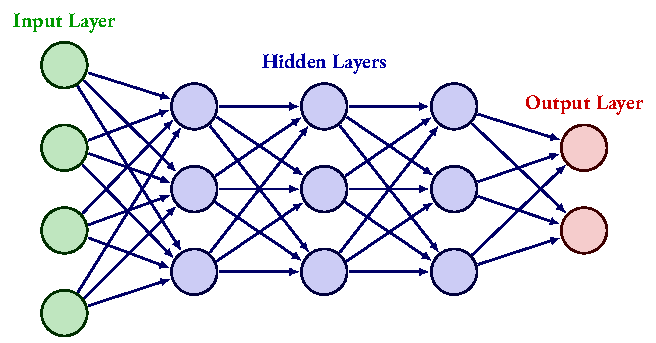
\includegraphics[scale=1.4]{tikz/chapter1 - Feedforward Neural Network.pdf}
    \caption{Example of a Feedforward Neural Network}
\end{figure}

A feedforward neural network can be thought of as a sequence of features, each of which represents a layer of the network. This structure is based on the composition of these functions to form an overall representation of the input data. Formally, we can represent a feedforward network as a composition of several functions:
$$ f(\mathbf{x}) = f^{(i)}(f^{(i-1)}(\dots f^{(2)}(f^{(1)}(\mathbf{x})) \dots )) $$  
Where \( f^{(1)} \) is the first layer (or input layer), \( f^{(i)} \) represents the output of the \(i\)-th layer, and so on. The depth of the network is defined by the number of layers, that is, the number of functions \( f^{(i)} \) involved.

In evaluating the functions of a feedforward network, which is acyclic graph, the flow of information proceeds in a single direction, from input to output. This flow passes through intermediate computations in the various layers of the network. 

In the initial layer, also called \textbf{\color{green!60!black}{Input Layer}}, each node corresponds to an input feature or variable, indeed there are no calculations or transformations applied to the data here.

Instead, neurons in the \textbf{\color{mybluee}{Hidden Layers}} perform nonlinear computations on the input data through the application of weights and activation functions.
The number of hidden layers and the number of neurons in each layer may vary depending on the architecture of the network and the complexity of the problem.
The main function of the hidden layers is to capture and represent complex and abstract features of the input data.

Finally in the \textbf{\color{red!80!black}{Output Layer}} we obtain the desired output.
The number of nodes in this layer depends on the nature of the problem, for example, in a binary classification problem there will be only one node, while in a multiclass classification problem there will be one node for each class.
Also the type of activation function used in the output layer depends on the type of problem the network is addressing! For example, for binary classification problems, the sigmoid activation function can be used, while for multiclass we use the softmax.

\subsection{Overcoming the limitations of linear models}

Linear models have long been used for their simplicity and convex optimization, but they have significant limitations in their ability to capture complex interactions between input variables. This limitation is particularly evident when dealing with complex problems such as nonlinear classification.

In the context of linear models, such as support vector machines, the choice of function \( \phi \) (\textbf{Nonlinear mapping of input data in feature space}) is crucial to satisfactory performance. However, there are limitations in engineering this function, which can make it difficult to capture complex information in the data. Below, we review three common options for addressing these challenges:
\begin{enumerate}
    \item \textbf{Use of generic \( \phi \)}: A first option is to use a generic \( \phi \) function. For example, in kernel machines with RBF (Radial Basis Function) kernels, \( \phi \) has implicit infinite dimensionality. This provides sufficient capacity to fit the training data. However, this approach may suffer from poor generalization for highly variable objective functions.
    \item \textbf{Engineer \( \phi \)}: Here, efforts are devoted to manually engineering a function that can capture the relevant information in the input data. However, this approach may be limited by the complexity of the data and the difficulty in correctly identifying key relationships.
    \item \textbf{Learning \( \phi \) from the data}: Finally, an option is to learn the \( \phi \) function directly from the data. This approach renounces convexity but offers significant advantages by combining the strengths of the first two options. \( \phi \) can be modeled very generically, and engineering can focus on designing neural network architectures capable of learning complex and informative representations from input data.
\end{enumerate}

Thanks to Feedforward Neural Networks we can overcome the limitations of traditional linear models because they are able to learn complex, nonlinear functions from data, thus overcoming the inherent limitations of linear models in capturing complex relationships between input variables.

The training of a neural network shares many similarities with that of other machine learning models. However, it has unique features that deserve to be explored. While it is essential to provide only the output of the final layers during training, the hidden layers do not require specific analysis during this phase, which contributes to the complexity and overall effectiveness of the network.

The main difference from linear models lies in the loss functions. While in linear models the loss is convex and guarantee convergence, in neural networks it become nonconvex, leading to greater complexity and not guaranteeing convergence to a global optimum.

Train a neural network means optimize the parameters' values $\mathbf{W}$ (wheights) in order to achieve $f(X,\mathbf{W})$ as close as the target unknown function $f(X)$. So, it is essential to apply gradient descent, an iterative approach to minimizing the cost function, and it is crucial to specify an appropriate \textbf{cost function} that accurately represents the error between the predicted output and the desired output. In addition, modeling choices may vary, including the selection of \textbf{output representation}, \textbf{activation functions}, and \textbf{network architecture} (e.g., number of layers), significantly affecting network performance.

Beyond that, there are other aspects of modeling that can be adapted to improve network performance, such as the choice of \textbf{optimizer} and the use of \textbf{regularization} techniques to avoid overfitting and improve generalization. 

To summarize, in a Neural Network we need to specify the following elements: cost function, output representation, activation function, architecture, optimizer, regularization.

\section{Cost Functions}

Cost (or Loss) functions play a key role in the training of deep learning models. They measure the \textbf{discrepancy between model predictions and actual target values} during the training process. An accurate choice of loss function is essential for optimal model performance.

For \textbf{Classification} problems, two commonly used loss functions are Categorical Cross-Entropy and Binary Cross-Entropy. These functions are designed to work with class probabilities and are particularly well suited for models that produce probability distributions.

{\Large
% $$
\begin{equation*}
\text{\textbf{Categorical Cross-Entropy}} = -\sum_{i=1}^{N} \tikzmarkk{Y}\textcolor{myred}{y_i} \log(\tikzmarkk{YC}\textcolor{mybluee}{\hat{y}_i})
\end{equation*}
\begin{tikzpicture}[overlay,remember picture]
    \node (Ye) [below of = Y, node distance = 3 em, anchor=west] {\footnotesize \textsf{\textcolor{myred}{true probability of class $i$}}};
    \draw[<-, in=180, out=-90] (Y.south)++(.25em,-1ex) to (Ye.west);

    \node (YCe) [below of = YC, node distance = 2 em, anchor=west] {\footnotesize \textsf{\textcolor{mybluee}{predicted probability of class $i$}}};
    \draw[<-, in=180, out=-90] (YC.south)++(.25em,-1ex) to (YCe.west);
\end{tikzpicture}
}

{\Large
% $$
\begin{equation*}
\text{\textbf{Binary Cross-Entropy}} = -\left(\tikzmarkk{Y}\textcolor{myred}{y}\log(\tikzmarkk{YC}\textcolor{mybluee}{\hat{y}}) + (1 - y) \log(1 - \hat{y})\right)
\end{equation*}
% $$
\begin{tikzpicture}[overlay,remember picture]
    \node (Ye) [below of = Y, node distance = 3 em, anchor=west] {\footnotesize \textsf{\textcolor{myred}{true label (0 or 1)}}};
    \draw[<-, in=180, out=-90] (Y.south)++(.25em,-1ex) to (Ye.west);

    \node (YCe) [below of = YC, node distance = 2 em, anchor=west] {\footnotesize \textsf{\textcolor{mybluee}{predicted probability of class 1}}};
    \draw[<-, in=180, out=-90] (YC.south)++(.25em,-1ex) to (YCe.west);
\end{tikzpicture}
}
\vspace{1cm}

In the case of \textbf{Regression}, different loss functions are used, including:

{\Large
% $$
\begin{equation*}
\text{\textbf{Mean Squared Error}} = \frac{1}{N} \sum_{i=1}^{N} (\tikzmarkk{Y}\textcolor{myred}{y_i} - \tikzmarkk{YC}\textcolor{mybluee}{\hat{y}_i})^2
\end{equation*}
% $$
\begin{tikzpicture}[overlay,remember picture]
    \node (Ye) [below of = Y, node distance = 3 em, anchor=west] {\footnotesize \textsf{\textcolor{myred}{actual (or true) target value for the example \( i \)}}};
    \draw[<-, in=180, out=-90] (Y.south)++(.25em,-1ex) to (Ye.west);

    \node (YCe) [below of = YC, node distance = 2 em, anchor=west] {\footnotesize \textsf{\textcolor{mybluee}{model prediction for the example \( i \)}}};
    \draw[<-, in=180, out=-90] (YC.south)++(.25em,-1ex) to (YCe.west);
\end{tikzpicture}
}
\vspace{1cm}

Mean Squared Error (MSE) calculates the mean squares of the differences between model predictions and actual values. It is commonly used and strongly penalizes significant errors. However, it is sensitive to outliers. 

% \newpage

{\Large
% $$
\begin{equation*}
\text{\textbf{Mean Absolute Error}} = \frac{1}{N} \sum_{i=1}^{N} |\tikzmarkk{Y}\textcolor{myred}{y_i} - \tikzmarkk{YC}\textcolor{mybluee}{\hat{y}_i}|
\end{equation*}
% $$
\begin{tikzpicture}[overlay,remember picture]
    \node (Ye) [below of = Y, node distance = 3 em, anchor=west] {\footnotesize \textsf{\textcolor{myred}{actual (or true) target value for the example \( i \)}}};
    \draw[<-, in=180, out=-90] (Y.south)++(.25em,-1ex) to (Ye.west);

    \node (YCe) [below of = YC, node distance = 2 em, anchor=west] {\footnotesize \textsf{\textcolor{mybluee}{model prediction for the example \( i \)}}};
    \draw[<-, in=180, out=-90] (YC.south)++(.25em,-1ex) to (YCe.west);
\end{tikzpicture}
}
\vspace{1cm}

Mean Absolute Error (MAE), or only Absolute Error (AE), calculates the mean of the absolute differences between predictions and actual values. It is less sensitive to outliers than MSE, but its derivative is undefined in zero.

{\Large
% $$
\begin{equation*}
\text{\textbf{Huber Loss}} = \frac{1}{N} \sum_{i=1}^{N} \left\{
\begin{array}{ll}
    \frac{1}{2} (y_i - \hat{y}_i)^2 & \text{se } |y_i - \hat{y}_i| \leq \textcolor{mygreen}{\delta} \\
    \tikzmarkk{D}\textcolor{mygreen}{\delta} (|y_i - \hat{y}_i| - \frac{1}{2} \textcolor{mygreen}{\delta}) & \text{otherwise}
\end{array}
\right.
\end{equation*}
% $$
\begin{tikzpicture}[overlay,remember picture]
    \node (De) [below of = D, node distance = 2.5 em, anchor=west]     {\parbox{\widthof{hyperparameter controlling the transition between}}{
    \ \\
    \footnotesize \textsf{\textcolor{mygreen}{hyperparameter controlling the transition between}} \\ 
    \footnotesize \textsf{\textcolor{mygreen}{the quadratic and linear regions of the loss function}}}};
    \draw[<-, in=180, out=-90] (D.south)++(.25em,-.5ex) to (De.west);
\end{tikzpicture}
}
\vspace{1cm}

Huber Loss combines the best features of MSE and MAE. For small errors, it behaves similar to MSE, while for larger errors, it behaves like AE. This avoids problems such as overfitting and steep slope of the MSE curve.

\textit{\textbf{Please Note}}: There are numerous other loss functions besides those mentioned above, which can be used depending on the specific problem to be addressed and the characteristics of the data. The choice of loss function depends on the goal of model training, the nature of the data, and the needs of the application. For example, in special contexts such as outlier detection or handling noisy data, specialized loss functions might be preferred. Moreover, as deep learning research advances, new loss functions are constantly being developed and existing ones adapted to meet emerging challenges in different application scenarios. 

\textit{\textbf{Also}}: The choice of the cost function is not independent of the choice of the output unit, because choosing one specific output unit over another can be convenient for the cost function we want to use (e.g., sigmoid and binary cross-entropy).

\section{Unit Types}

\subsection{Linear Units}

Linear Units play a key role in the intermediate and output layers of neural networks. These units apply a \textbf{linear transformation to the inputs} by combining the weights associated with the inputs with the input values themselves. The output produced by Linear Units is a linear combination of the inputs. 

The formula for calculating the output of Linear Units is:
$$
\hat{y} = W^T h + b
$$
Where \( \hat{y} \) represents the predicted output, \( W \) are the weights associated with the inputs, \( h \) represents the features from the previous layer, and \( b \) is the bias term.

\subsection{Softmax Units}

Softmax Units are commonly used in the output layers of neural networks, especially in cases of Multiclass Classification (with Cross-Entropy Loss). These units transform the un-normalized scores from the last linear layer into a \textbf{normalized probability distribution}, allowing the model to assign a probability to each membership class for a given input.

The softmax formula used to calculate the probabilities is as follows:
$$
\text{Softmax}(z_i) = \frac{e^{z_i}}{\sum_{j} e^{z_j}}
$$
Where \( z_i \) represents the non-normalized score associated with the class \( i \), and \( \sum_{j} e^{z_j} \) is the sum of all the exponents of the non-normalized scores.

Log Softmax is a variant of the Softmax function that is used to \textbf{improve numerical stability} when computing probabilities. The formula for calculating the Log Softmax is as follows:
$$
\text{log Softmax}(z_i) = z_i - \log\left(\sum_{j} e^{z_j}\right)
$$

Here are some advantages:
\begin{itemize}
    \item \textbf{The term \( z_i \) never saturates}: This means that the scale of values \( z_i \) is not compressed or restricted in any way. This is beneficial because it allows the model to continue to learn from more relevant information without limitations imposed by value saturation.
    
    \item \textbf{Maximizing the log-likelihood encourages \( z_i \) to be increased, while encouraging all other \( z \) to be decreased}: When we maximize the log-likelihood, we are trying to make the model's prediction as close to reality as possible. Thus, we encourage \( z_i \) to increase, since it represents the probability associated with the correct class. At the same time, we encourage the other \( z \) to decrease to reduce the probability associated with the wrong classes.
    
    \item \textbf{The log-likelihood cost function heavily penalizes the most active incorrect prediction}: The log-likelihood cost function significantly penalizes the most active incorrect prediction. This means that if the model is very sure of an incorrect prediction (for example, it has a very high probability for an incorrect class), the cost function will increase significantly, encouraging the model to correct that error.
\end{itemize}

This analysis prompts us to consider a fundamental question: \textit{How can we select the activation function $h$ most suitable for our neural network?}

In the next section, we try to answer this crucial question! 
We have decided to be quite descriptive, as we believe that more details about these functions can facilitate a deeper understanding.

\section{Activation Functions}

\subsection{Sigmoid}

\begin{table}[h]
\begin{tabularx}{\linewidth}{>{\parskip1ex}X@{\kern4\tabcolsep}>{\parskip1ex}X}
\toprule
\hfil\bfseries \color{mybluee}{Pros}
&
\hfil\bfseries \color{mybluee}{Cons}
\\\cmidrule(r{3\tabcolsep}){1-1}\cmidrule(l{-\tabcolsep}){2-2}

%% PROS
The sigmoid function offers a valuable advantage because it acts as a type of \textbf{\textcolor{mybluee}{squashing non-linearity}} that "squeezes" outputs within the range of [$0$, $1$]. This feature is particularly advantageous in scenarios such as binary classification tasks, where the model must generate outputs that can be interpreted as probabilities.

Moreover, the sigmoid function has a property of \textbf{\textcolor{mybluee}{differentiability and smoothness}} over its entire domain. This property facilitates seamless integration with gradient-based optimization techniques, ensuring stable convergence during the training process.
&

%% CONS
However, it \textbf{\textcolor{mybluee}{tends to saturate}} in most of its domain. This saturation phenomenon causes the gradient to tend toward zero, posing challenges during the learning phase. Consequently, this saturation can obstruct the effective propagation of gradients through the network during back-propagation.

In addition, the sigmoid function shows strong sensitivity mainly when the input is near zero. In contrast, its \textbf{\textcolor{mybluee}{sensitivity decreases}} for both large and small input values. This characteristic negatively affects the model's ability to learn from datasets that have a wide range of input values.
\\\bottomrule
\end{tabularx}
\caption{Benefits and Limitations of Sigmoid Activation}
\end{table}

\vspace{1cm}
\begin{figure}[!htbp]
    \centering
    \includegraphics[scale=2]{tikz/chapter1 - Sigmoid.pdf}
    \caption{Sigmoid Activation Function Plot}
\end{figure}

\newpage
\subsection{Hyperbolic Tangent}

\begin{table}[h]
\begin{tabularx}{\linewidth}{>{\parskip1ex}X@{\kern4\tabcolsep}>{\parskip1ex}X}
\toprule
\hfil\bfseries \color{myred}{Pros}
&
\hfil\bfseries \color{myred}{Cons}
\\\cmidrule(r{3\tabcolsep}){1-1}\cmidrule(l{-\tabcolsep}){2-2}

%% PROS
First, it is \textbf{\textcolor{myred}{differentiable and continuous}}, ensuring compatibility with gradient-based optimization techniques. 

In addition, the hyperbolic tangent function is \textbf{\textcolor{myred}{similar to sigmoid}}, but provides a more favorable output range. By squashing the outputs in the interval [$-1$, $1$], it ensures that the outputs are centered in zero. This feature can improve the model's ability to learn and adapt to data distributions, especially in scenarios where centered data is advantageous.
&

%% CONS
However, the hyperbolic tangent function also has limitations. Like the sigmoid, it tends to \textbf{\textcolor{myred}{saturate}} throughout much of its domain. This saturation phenomenon can hinder effective gradient propagation during back-propagation, impeding the learning process and potentially leading to slower convergence.
\\\bottomrule
\end{tabularx}
\caption{Benefits and Limitations of Hyperbolic Tangent Activation}
\end{table}

\vspace{1cm}
\begin{figure}[!htbp]
    \centering
    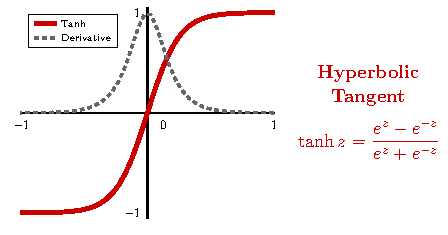
\includegraphics[scale=2]{tikz/chapter1 - Hyperbolic Tangent.pdf}
    \caption{Hyperbolic Tangent Activation Function Plot}
\end{figure}

\newpage
\subsection{Rectified Linear Unit (ReLU)}
\begin{table}[h]
\begin{tabularx}{\linewidth}{>{\parskip1ex}X@{\kern4\tabcolsep}>{\parskip1ex}X}
\toprule
\hfil\bfseries \color{mygreen!80!black}{Pros}
&
\hfil\bfseries \color{mygreen!80!black}{Cons}
\\\cmidrule(r{3\tabcolsep}){1-1}\cmidrule(l{-\tabcolsep}){2-2}

%% PROS
The ReLU function has several advantages. First, it provides \textbf{\textcolor{mygreen!80!black}{wide and consistent gradients}} when it is active. This means that the ReLU function does not saturate when it is active, which greatly accelerates the convergence of gradient-based optimization.
In addition, the \textbf{\textcolor{mygreen!80!black}{non-positive limitation}} accelerates the convergence of gradient descent, allowing for faster learning.
The ReLU function may have a limitation in its \textbf{\textcolor{mygreen!80!black}{differentiability}}. However, in practice, this is not necessarily a problem since the one-sided derivative is returned when \( z = 0 \). Moreover, gradient-based optimization is subject to numerical errors anyway, so this differentiability limitation is often overlooked.
A good practice is to \textbf{\textcolor{mygreen!80!black}{initialize bias}} with small positive values. This ensures that units are initially active for most inputs and that derivatives can propagate through.
&

%% CONS
However, the ReLU function also has some disadvantages. First of all, its outputs are not \textbf{\textcolor{mygreen!80!black}{centered on zero}}, which could cause problems in some machine learning contexts.
In addition, ReLU neurons may suffer from a phenomenon called \textbf{\textcolor{mygreen!80!black}{"dying ReLU"}}. This occurs when most of the inputs to ReLU neurons are in the negative range. When this occurs, the ReLU neurons return an output of $0$ and the gradients do not flow during back-propagation, preventing the weights from updating. However, this problem does not always occur and can be mitigated by properly adjusting the learning rate or using Stochastic Gradient Descent (SDG).
The ReLU function can also be sensitive to the \textbf{\textcolor{mygreen!80!black}{large learning rate}}. If the learning rate is too high, the new weights are likely to end up in the highly negative range, negatively affecting the convergence of the model.
\\\bottomrule
\end{tabularx}
\caption{Benefits and Limitations of ReLU Activation}
\end{table}

\vspace{1cm}
\begin{figure}[!htbp]
    \centering
    \includegraphics[scale=2]{tikz/chapter1 - ReLU.pdf}
    \caption{ReLU Activation Function Plot}
\end{figure}


\subsection{Generalized Rectified Linear Units}

The \textbf{generalized rectified linear units} were introduced to address some limitations of the ReLU function. The main objective is to obtain a non-zero slope when \( z_i < 0 \). The generalized form of the ReLU is defined as follows:
$$ h(z, \alpha_i) = \max(0, z_i) + \alpha_i \min(0, z_i) $$
However, generalized rectified linear units are not universally better than ReLU and may lead to other problems, such as additional computational complexity. Some of the improvements that have been made include:
\begin{itemize}     
    \item \textbf{Leaky ReLU}: This variation solves the problem of neuron death by setting \( a_i \) to a small value, such as $0.01$, to maintain a gradient flow even when the input is negative.
    \item \textbf{Parametric ReLU}: This variant allows the parameter \( a_i \) to be learned, allowing the network to adapt the gradient of the activation function based on the data.
    \item \textbf{ReLU Randomized}: This variant samples the parameter \( a_i \) from a fixed interval during training and keeps it constant during testing, introducing randomness into the model.
\end{itemize}

In addition, other activation functions have been proposed as alternatives to ReLU, including:
\begin{itemize}     
    \item \textbf{Exponential Linear Units (ELU)}: This activation function retains all the advantages of ReLU but avoids the problem of neuron death. However, it requires exponentiation during computation, slightly increasing the computational complexity.
    \item \textbf{Swish}: This function is a smooth, non-monotonic function that has been shown to perform better than ReLU on deeper models, improving performance on datasets such as ImageNet.
    \item \textbf{Linear Units with Gaussian Error (GELU)}: This activation function has been used in state-of-the-art algorithms such as GPT-3 and BERT. It combines the non-monotonic aspect (that helps for the gradient of the function),  regularization techniques such as dropout and zone-out, and ReLU benefits to achieve a smoother version of ReLU. 
\end{itemize}

% These improvements and generalizations of activation functions have helped make neural networks more efficient and adaptable to a wide range of machine learning problems. Below, we show graphs of the Leaky ReLU and ELU activation functions for a better understanding of their properties.

\begin{figure}[!htbp]
    \centering
    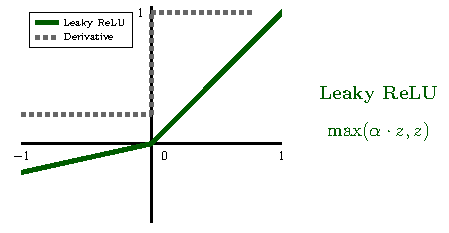
\includegraphics[scale=2]{tikz/chapter1 - Leaky ReLU.pdf}
    \caption{Leaky ReLU Activation Function Plot}
\end{figure}

\begin{figure}[!htbp]
    \centering
    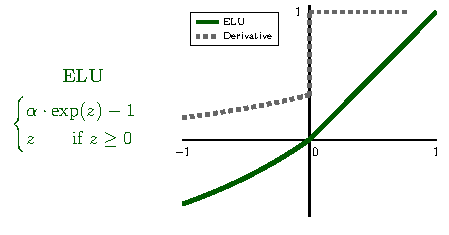
\includegraphics[scale=2]{tikz/chapter1 - ELU.pdf}
    \caption{ELU Activation Function Plot}
\end{figure}

\section{Architecture design}
\textit{How do we decide depth and width?} Choosing the depth and width of a neural network depends on several factors, including the complexity of the problem to be solved, the availability of training data, and the computational resources available. In principle, how many hidden layer units are sufficient? Theory offers us some answers.

\begin{remark}
Cybenko's Theorem (1989), also known as the universal approximation theorem, states that \textbf{a two-layer neural network with linear output can approximate any continuous function} over a compact domain with arbitrary precision, provided there are enough hidden units. This theorem has important implications for the design of neural architectures.
\end{remark}

\textbf{Implications}: Regardless of the function we are trying to learn, we know that a large multilayer neural network can represent this function. However, there is no guarantee that our training algorithm will be able to learn that function, due to optimization or data overlap issues. Also, the theorem gives no indication of how large the network will be.

\textit{So is depth or width more important?} There are trade-offs between depth and width of neural networks. For example, deeper networks generally generalize better: imagine a neural network as a set of tools to solve a problem. The more tools you have, the more complex problems you can solve. Then, by adding more "layers" to the network (making it deeper), we could give the network the ability to tackle more difficult problems or capture finer details in the data. In addition, architecture design has a significant impact on performance, for example between convolutional and feedforward neural networks.

% \newpage
% \chapter{Lorem} \label{ch:lorem}
% \section{Proin nec metus venenatis} \label{sec:proin}

Condimentum quam sed, auctor diam. Fusce at bibendum nunc. Vestibulum ut justo
volutpat, placerat turpis at, ultrices lacus. Phasellus blandit fermentum tincidunt.

Quisque eget est ullamcorper massa vestibulum facilisis eget non quam. Pellentesque
eleifend augue vel elit mattis, ut porta risus sodales. Suspendisse vitae odio
facilisis, venenatis leo ut, consequat turpis.

\subsection{Integer magna quam}

In hac habitasse platea dictumst. Pellentesque a hendrerit mauris, ac congue
erat. Maecenas in lorem non velit euismod volutpat. Morbi et arcu quam. Mauris
id scelerisque est. Cras a nunc in justo blandit dictum nec ut tortor.

\begin{figure}[hb]
\centering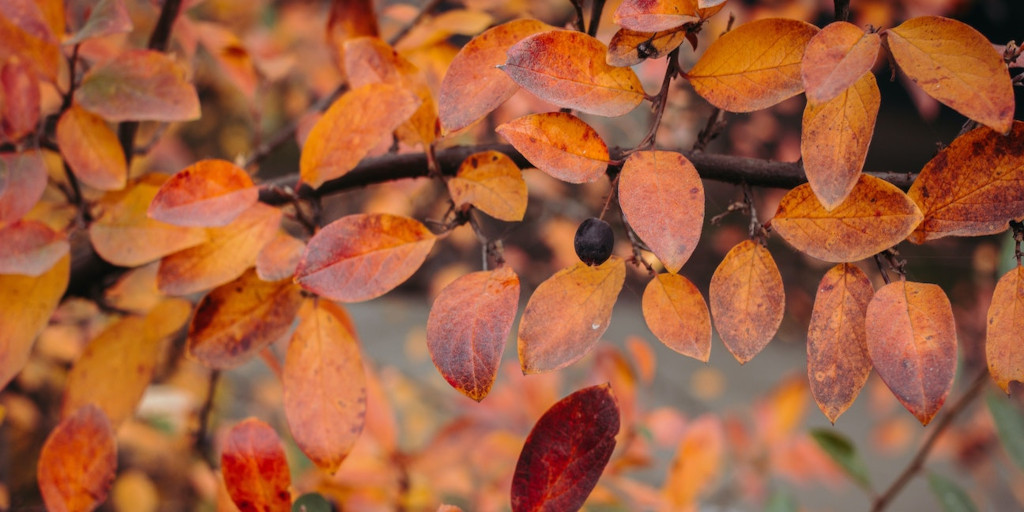
\includegraphics[scale=1]{images/orange2.jpg}
\caption{Maecenas varius orci vitae eros euismod placerat} \label{fig:integer}
\end{figure}

\subsection{Convallis quis elementum feugiat}

Rutrum in ligula. Nulla ut semper ligula, sed lobortis enim. Vivamus nulla eros,
faucibus ac convallis in, ornare at elit. Aliquam erat odio, finibus at purus ut,
porta ullamcorper odio. Vivamus ac augue tincidunt, semper magna volutpat,
condimentum sem. Praesent eget neque vitae odio volutpat vulputate.


\newpage 
\section{Phasellus} \label{sec:phasellus}

Lorem ipsum \textbf{dolor sit amet}, consectetur adipiscing elit. Aliquam eu nibh non
tortor maximus tincidunt. Sed pellentesque lacus a metus pellentesque, vel
ultrices leo pulvinar. Ut finibus ipsum ornare, vehicula mauris id, pulvinar
enim. Proin in neque elit. Duis eget tempus turpis. Ut consectetur lacinia
augue pulvinar bibendum. Nulla sed nulla ut mauris consequat egestas ac et orci.

\subsection{Suspendisse potenti}

Integer venenatis, \textit{lectus a dapibus vehicula}, diam odio rutrum ante, at dictum
erat lorem et sapien.

Suspendisse potenti :

\begin{itemize}
\item{pellentesque habitant morbi tristique}
\item{senectus et netus et malesuada fames ac turpis egestas}
\item{ut sit amet ultricies nisl}
\item{etiam laoreet condimentum lacus et elementum}
\end{itemize}

Sed vehicula quis ligula non fermentum. Pellentesque semper ligula gravida "$C_i$",
bibendum dui ut, semper nibh. Quisque a risus porta, fermentum velit vitae,
pellentesque felis.

\newpage
\subsection{Phasellus et quam}

Suspendisse potenti. Aliquam id metus in purus imperdiet aliquam eu ut dolor :

\begin{highlight}
\begin{align}
\alpha_{i+1} &= \frac{A_{i+1}}{S_{i+1}} \\
             &= \frac{A_i + \Delta A_i}{S_i + \Delta S_i} \\
             &= \frac{A_i + \Delta A_i}{S_i + \frac{\Delta A_i}{\alpha_i}} \\
             &= \alpha_i * \frac{A_i + \Delta A_i}{\alpha_i * S_i + \Delta A_i} \\
             &= \alpha_i
\end{align}
\end{highlight}

Vestibulum luctus consectetur vestibulum. Duis ullamcorper ligula nec mauris
viverra rhoncus. Aliquam auctor est accumsan odio vehicula ornare.

\begin{remark}
Duis et metus auctor, fringilla nulla non, dapibus felis \ref{sec:proin}.
\end{remark}

Morbi ipsum dui, rutrum et cursus a, porta eu ligula. Nulla lobortis leo eget
odio bibendum rhoncus. Maecenas posuere nulla nec felis viverra blandit.

\subsection{Felis nunc}

Sit amet elementum tortor malesuada quis. Quisque pellentesque nisl quis augue
interdum vehicula. Nunc nec dictum sem. Nunc venenatis elementum hendrerit \href{https://example.com/}{example.com}.

\begin{remark}
Pellentesque ut justo arcu. Fusce cursus luctus tortor eu venenatis.
\end{remark}

Maecenas viverra dui vitae eros tristique, porta elementum mi aliquam. Cras
sodales erat et molestie auctor. Phasellus mauris eros, bibendum sit amet
rhoncus id, bibendum ut velit.


\section*{Integer semper dictum tellus}

Neque eu cursus faucibus, ipsum magna tincidunt dui, vel scelerisque urna nibh ut nisl:

\begin{description}[labelwidth=\widthof{\bfseries morbi convallis},align=left]
\item[Duis]{sit amet mattis magna.}
\item[Curabitur]{sit amet fermentum mi.}
\item[Morbi convallis]{purus eu fermentum accumsan, mauris felis consequat ipsum.}
\item[Ut]{sollicitudin sit amet tellus et mollis.}
\end{description}

\section*{A porttitor orci faucibus sit amet}

Vivamus et sapien vitae lacus ornare suscipit vitae id mauris:

\begin{description}[labelwidth=\widthof{\bfseries suspendisse},align=left]
\item[Vivamus]{in dui arcu.}
\item[Morbi]{vitae dolor libero.}
\item[Tellus]{est, pellentesque at ultrices non, consectetur sit amet augue.}
\item[Suspendisse]{elementum mollis nisl at aliquam.}
\end{description}

\newpage 
\section{Ipsum primis}

In faucibus orci luctus et ultrices posuere cubilia curae; Aliquam nunc ipsum,
sollicitudin ut tempus consectetur, fermentum at lectus.

Nullam molestie viverra augue sit amet gravida.

\newenvironment{nomenclature}[1]
{
\begin{table}[hbt]
\caption{#1}
\begin{center}
\begin{tabular}{|l|l|l|}
\hline
\textbf{Symbol} & \textbf{Unit} & \textbf{Description}\\
\hline
}
{
\\\hline
\end{tabular}
\end{center}
\end{table}
}

\subsection{Mauris pellentesque}

\begin{nomenclature}{Massa sagittis malesuada}
$g$     & $m/s^{2}$ & nisi in mollis gravida
\end{nomenclature}

\subsection{Nulla massa}

\begin{nomenclature}{Quis imperdiet}
$Q_{p}$         & $t/h$             & consectetur tortor
\end{nomenclature}

\begin{nomenclature}{Magna lectus}
$\tau_{a}$    	& $^{\circ}C$       & integer mollis bibendum gravida\\
$f_{s}$     	& $/jour$           & vestibulum porta urna at ex dignissim tincidunt
\end{nomenclature}

\subsection{Nam vitae}

\begin{nomenclature}{Nibh a lacus tincidunt efficitur}
$X_n$   & $m$               & venenatis nisi\\
$Y_n$   & $m$               & integer malesuada eu ligula nec pharetra\\
$Z_n$   & $m$               & fusce non elit lectus
\end{nomenclature}


\newpage 
\section{Phasellus tristique} \label{sec:phasellus-tristique}

Lacus ac turpis semper fringilla. Mauris fermentum varius neque, vel congue
elit tempus quis. Aliquam a nunc in nunc consectetur hendrerit ut quis felis. 

Quisque id dui magna. Curabitur posuere nisl at magna vehicula aliquam \ref{fig:duis}.
Duis et suscipit felis. Mauris non justo quis diam gravida placerat condimentum
ut sapien. Praesent imperdiet libero id est tincidunt ullamcorper.

\begin{figure}[ht]
\hspace*{-1.6cm}
\begin{tikzpicture}

\node (logs) [io] {Logs};
\node (storage) [io, right=2cm of logs] {Storage};
\node (log-topics) [io, below=1cm of logs] {Log: topics, data};

\node (parse-data) [block, below=1cm of log-topics] {Parse event arguments};
\node (arguments) [io, below=2.7cm of parse-data] {Event arguments};

\node (parse-selector) [block, left=2cm of parse-data] {Parse event selector};
\node (reverse-selector) [block, below=1cm of parse-selector] {Reverse selector};
\node (signature) [io, below=1cm of reverse-selector] {Event signature};

\node (identify-standard) [block, below=1cm of signature] {Identify standard and event};
\node (fetch-constraints) [block, below=1cm of identify-standard] {Fetch matching constraints};
\node (check-constraints) [decision, below=4.3cm of arguments] {Constraints?};

\node (references) [io, left=1.6cm of identify-standard] {References};
\node (rules) [io, left=2cm of fetch-constraints] {Rules};

\node (negative) [io, below=2cm of check-constraints] {False};
\node (positive) [io, right=2cm of negative] {True};

\node (c1) [container, fit=(parse-selector) (reverse-selector) (parse-data), draw=gray] {};

\node (c2) [container, fit=(identify-standard) (fetch-constraints), draw=gray] {};

\node (c3) [container, fit=(positive) (negative)] {};

\node (c4) [container, fit=(references) (rules)] {};

\node (c0) [container, fit=(log-topics) (c1) (c2) (check-constraints), inner ysep=6mm, yshift=-2mm] {};
\node (t0) [label, above=2mm of c0, xshift=-4cm] {Event poisoning?};

\draw [arrow] (logs) -- (log-topics);
\draw [arrow] (log-topics) -| (parse-selector);
\draw [arrow] (log-topics) -- (parse-data);
\draw [arrow] (parse-selector) -- (reverse-selector);
\draw [arrow] (reverse-selector) -- (signature);
\draw [arrow] (signature) -- (identify-standard);
\draw [arrow] (parse-data) -- (arguments);
% \draw [arrow] (arguments) |- (identify-standard);
\draw [arrow] (arguments) -- (check-constraints);
\draw [arrow] (identify-standard) -- (fetch-constraints);
\draw [arrow] (fetch-constraints) |- (check-constraints);
\draw [arrow] (references) -- (identify-standard);
\draw [arrow] (rules) -- (fetch-constraints);
\draw [arrow] (storage) -- +(0,-9cm) -| (check-constraints);
\draw [arrow] (check-constraints) -| node[label, near start, above] {no} (positive);
\draw [arrow] (check-constraints) -- node[label, near start, right] {yes} (negative);

\draw [arrow] (logs) edge [loop above] node[label, above] {Iterate} ();

\end{tikzpicture}
\caption{Maecenas hendrerit congue faucibus} \label{fig:duis}
\end{figure}

\newpage 
\section{Sed ultrices} \label{sec:sed-ultrices}

\subsection{Donec pellentesque}

Tempus ipsum, vitae condimentum nisi efficitur id. In velit mauris, auctor eget
sapien nec, viverra mattis neque. Nunc vel commodo nunc, eget cursus ex.

\begin{enumerate}
\item{Nunc maximus consequat tristique.}
\item{Praesent luctus ex aliquam rhoncus consectetur.}
\item{Suspendisse mattis velit ante, vitae mollis est pharetra a.}
\item{Duis tincidunt, urna id auctor imperdiet, odio dui ullamcorper nisi.}
\item{Integer tincidunt enim vitae nulla iaculis, in varius metus blandit.}
\item{Nunc quam arcu, fermentum non dapibus condimentum, condimentum eget nunc.}
\end{enumerate}

\subsection{Euismod sodales}

\begin{outline}
\lipsum[2]
\end{outline}

\subsection{Pellentesque a nulla}

\begin{lstlisting}[language=Solidity]
contract KingOfTheHill is Ownable {
    address public owner; // different from the owner in Ownable

    function () public payable {
        if(msg.value > jackpot) owner = msg.sender; // local owner
        jackpot += msg.value;
    }
    function takeAll () public onlyOwner { // contract creator
        msg.sender.transfer(this.balance);
        jackpot = 0;
    }
}
\end{lstlisting}


\newpage
\
\newpage
\listoffigures
\listoftables
%----------------------------------------------------------------------------------------
% \newpage
% \printbibliography[title = {Aliquam}]

\end{document}